\section*{Algorithms}
We chose to implement SHA-1 in OpenCL as a baseline to see how well the NIST competitors have been able to include parallelism in their designs.
Additionally, we implemented a subset of the current round 2 SHA-3 candidate algorithms: the CubeHash, ECHO, and Skein algorithms.

\subsection*{CubeHash}

CubeHash was designed by Daniel J. Berstein--a big name in the cryptography community.
It is perhaps the simplest SHA-3 candidate and, as such, as garnered significant attention.
CubeHash can be parameterized on the number of rounds $r$, the number of bytes per block $b$, and the number of desired output bits $h$.
For our tests, we chose $r=16$, $b=32$, and $h=512$ primarily because these were the recommended parameters specified by the author~\cite{CubeHash-spec}.

Internally, CubeHash maintains a 1024-bit state that is transformed $r$ times every $b$ bytes.
The transformation is simply a series of additions, swaps, rotations, and xors, thus making it easy to verify.
To output a hash, the internal state is truncated to the desired number of bits.
Thus, the runtimes for different $h$s should be relatively similar.
The authors of the algorithms estimate their algorithm can run 20 cycles/byte on the NIST reference platform for the parameters specified above~\cite{Bernstein}.

\subsection*{ECHO}
ECHO was designed by the Crypto Research Group.
ECHO is based largely on the AES block cipher chosen by NIST to replace the defunct Data Encryption Standard as an official federal government standard in the United States.
ECHO provides a number of advantages over other hash functions in the competition because is built upon the AES block cipher.
In particular, Intel chips starting with the current Nehalem core will have built in AES hardware support - allowing for three times faster operation than previous general purpose CPU chips.\cite{Westmere}
In addition to receiving performance enhancements from any AES optimizations built into hardware, testing ECHO on a GPU should also give some indication of how effective running AES as a GPGPU program would be.
Preliminary results from researchers have demonstrated up to a 2-20x increase in encryption rate throughput by using the GPU as a encryption co-processor~\cite{Harrison}, \cite{Manavski}.
However, there is good reason to doubt the 20x figure as it appears that it was achieved through a naive implementation of AES using Electronic Code Book (ECB) mode.
Unlike more secure encryption modes, ECB mode encrypts data in finite sized chunks allowing for easy data parallelization.  
However, because this results in each portion of the ciphertext being encrypted independently of one another - ECB mode is largely insecure for many use cases~\cite{CodeBook}.

\begin{figure}[htp]
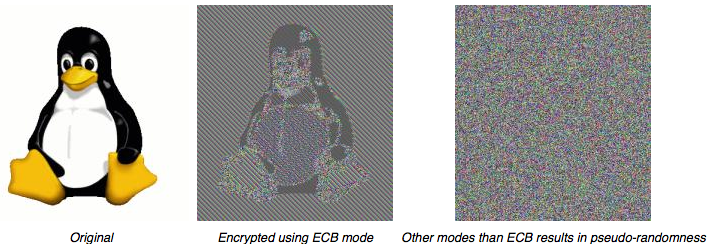
\includegraphics[width=\textwidth]{../data/ECB.png}
\caption{Encrypting any file with inherent structure - like a picture - demonstrates the weakness of ECB mode encryption.\cite{CodeBook}}\label{fig:ecb}
\end{figure}

ECHO runs 8 rounds, each round consists of 2 AES rounds.
Additionally, ECHO uses a ShiftRows function similar to AES but on 128 bit words, and AES's MixColumns on 4-tuples.
The only parameter to specify for ECHO is the hash length - we chose a length of 512 bits for our tests - but also ran a test with varied hash length to compare against CubeHash.

\subsection*{Skein}

Skein was designed by Niels Ferguson and Bruce Schneier--big names in the cryptography and security community.
Skein is based on the Threefish block cipher and supports internal block sizes of 256, 512 or 1024 bits and runs in 72 or 80 rounds.
Skein allows for arbitrary digest size, was designed for 64 bit processors and speed was a primary consideration of the design.
According to the authors, Skein can run at 6.1 cycles/byte on a Core 2 Duo in 64 bit mode~\cite{SkeinSpeed}.
This means, in theory, that Skein can run faster than even SHA-1 or SHA-2 while providing much greater security.
Skein also has a number of optional features or alternate implementation modes which can allow for use as a ``a PRNG, a stream cipher, a key derivation function, authentication without the overhead of HMAC''\cite{SkeinSpeed}.
It also has an optional hash-tree mode for increasing parallel execution speed, however there is not yet an implementation of this mode. 

